\documentclass[11pt,a4paper]{article}
\usepackage[a4paper, portrait, margin=1in]{geometry}
\usepackage[utf8]{inputenc}
\usepackage[T1]{fontenc} 
\usepackage{graphicx}
\usepackage{booktabs}
\usepackage{enumitem}
\usepackage{pdfpages}
\usepackage{mathptmx}
\usepackage{anyfontsize}
\usepackage{titlesec}
\usepackage{tabto}
\usepackage{listings}

%\usepackage[table,xcdraw]{xcolor}
% If you use beamer only pass "xcolor=table" option, i.e. \documentclass[xcolor=table]{beamer}
\usepackage[normalem]{ulem}
\useunder{\uline}{\ul}{}

\usepackage{xcolor}

\definecolor{codegreen}{rgb}{0,0.6,0}
\definecolor{codegray}{rgb}{0.5,0.5,0.5}
\definecolor{codepurple}{rgb}{0.58,0,0.82}
\definecolor{backcolour}{rgb}{0.95,0.95,0.92}

\lstdefinestyle{mystyle}{
    backgroundcolor=\color{backcolour},   
    commentstyle=\color{codegreen},
    keywordstyle=\color{magenta},
    numberstyle=\tiny\color{codegray},
    stringstyle=\color{codepurple},
    basicstyle=\ttfamily\footnotesize,
    breakatwhitespace=false,         
    breaklines=true,                 
    captionpos=b,                    
    keepspaces=true,                 
    numbers=left,                    
    numbersep=5pt,                  
    showspaces=false,                
    showstringspaces=false,
    showtabs=false,                  
    tabsize=2
}

\lstdefinelanguage{JavaScript}{
  keywords={typeof, new, true, false, catch, function, return, null, catch, switch, var, if, in, while, do, else, case, break},
  keywordstyle=\color{blue}\bfseries,
  ndkeywords={class, export, boolean, throw, implements, import, this},
  ndkeywordstyle=\color{darkgray}\bfseries,
  identifierstyle=\color{black},
  sensitive=false,
  comment=[l]{//},
  morecomment=[s]{/*}{*/},
  commentstyle=\color{purple}\ttfamily,
  stringstyle=\color{red}\ttfamily,
  morestring=[b]',
  morestring=[b]"
}

\lstdefinelanguage{XML}
{
  morestring=[b]",
  morestring=[s]{>}{<},
  morecomment=[s]{<?}{?>},
  stringstyle=\color{black},
  identifierstyle=\color{blue},
  keywordstyle=\color{cyan},
  morekeywords={xmlns,version,type}
}
\lstset{language=C++,
                keywordstyle=\color{blue},
                stringstyle=\color{red},
                commentstyle=\color{green},
                morecomment=[l][\color{magenta}]{\#}}

\lstset{style=mystyle}

\usepackage{tocbasic}

\DeclareTOCStyleEntry[
  entrynumberformat=\entrynumberwithprefix{\figurename},
  dynnumwidth,
  numsep=1em
]{tocline}{figure}
\newcommand\entrynumberwithprefix[2]{#1\enspace#2:\hfill}

\usepackage{hyperref}
\hypersetup{
  colorlinks,
  allcolors=.,
  urlcolor=blue,
}

\usepackage{setspace}
\setcounter{secnumdepth}{4}
\titleformat{\paragraph}
{\normalfont\normalsize\bfseries}{\theparagraph}{1em}{}
\titlespacing*{\paragraph}
{0pt}{3.25ex plus 1ex minus .2ex}{1.5ex plus .2ex}

\usepackage{tikz}
\usepackage{amsmath}
\usetikzlibrary{shapes.geometric, arrows}
\usepackage{verbatim}
\usepackage{array}
\usepackage{caption}
\pagestyle{plain}
\setlength{\parindent}{0pt}
\renewcommand{\thesection}{\arabic{section}}

\hyphenpenalty 1000
\exhyphenpenalty 1000


\begin{document}


\begin{titlepage}

    \begin{center}
    
        {\fontsize{22}{27}\selectfont Department of Electronic and Telecommunication Engineering} 
	\vspace{\baselineskip}
	\vspace{\baselineskip}
        {\fontsize{20}{24}\selectfont \\Internet of Things}  
        {\fontsize{16}{19}\selectfont \\EN3250} 
    \vspace{\baselineskip}
	\vspace{\baselineskip}
        {\fontsize{20}{24}\selectfont \\Currency Converter Service}  
	   {\fontsize{18}{21}\selectfont \\Project Report\\} 
%		\vspace{\baselineskip}
%		\vspace{\baselineskip}   
%		\vspace{\baselineskip}
%		\vspace{\baselineskip}
		\vspace{\baselineskip}
    \end{center}

   \begin{center}
        
\includegraphics[width=0.4\textwidth]{images/uom.png}
    \end{center}
   \begin{center}   
      {\fontsize{16}{19}\selectfont University of Moratuwa\\}   
      \vspace{\baselineskip}
    \end{center}

\begin{flushleft}

{\fontsize{16}{19}\selectfont
\NumTabs{7}

\setlength{\itemindent}{1.7in}
\item 170258L 
      \tab
      :  R.H.R.  Jayarathne
\item 170543G
      \tab
      :  M.K.T. Sampath
 
\item 170698J
      \tab
      :  L.T.A. Wijayaratne

\item 170375R
      \tab
      :  D.R. Marasinghe


}
\end{flushleft}


\begin{center}
\vspace{\baselineskip}
\vspace{\baselineskip}
\vspace{\baselineskip}
\vspace{\baselineskip}
\vspace{\baselineskip}
\vspace{\baselineskip}
\vspace{\baselineskip}


 {\fontsize{10}{13}\selectfont This report is submitted in partial fulfilment of the requirements for the module}\\
  {\fontsize{10}{13}\selectfont EN3250 - Internet of Things}
 \end{center} 

\end{titlepage}



 




	

\pagenumbering{roman} 
\spacing{1.45} 
\newpage
\tableofcontents



\newpage
\section{Introduction}

\subsection{Overview}

Foreign exchange market is a global market, where people around the world buy and sell different foreign currencies everyday for various purposes. One purpose of the traders in the market is engaging in day-trading activities. Day trading is performed by normal people who intend to obtain profits and earn out of small price mismatches that are available for a short amount of time. Day traders’ activity is influenced by information generated from past foreign currency price information. This information is generated by performing various kinds of mathematical transformations on time series price charts . These people find a lot of value in this information generated and they usually buy required market information from their trusted services.

This project mainly focuses on providing foreign exchange market day-traders, a selected set of useful information. This is achieved by using a currency API that provides live currency prices of various currencies around the world. Usually, hourly past currency price data are not available easily, because past currency data is usually provided on a daily basis. Due to this reason, storing the live currency data in the database is useful for making predictions. Users will also find the notification system that warns when the prices are beginning to exceed their expected boundaries, valuable.

ESP8266 is used for controlling the display as well as connecting to the user’s mobile phone and Node-Red through WiFi technology. Node-Red to Node-MCU communication happens through the MQTT communication protocol. Node-MCU’s ability to enter into sleep mode is also utilized. Node-MCU acts as both Wifi access point and http server. The user may sign-in using a username and a password, when the Node-MCU is functioning as a server. The access point mode is required when it is fetching and submitting data.


\subsection{Objectives}

\begin{itemize}[itemsep=-1.7mm]

\item To provide several technical analysis charts such as Simple Moving Average \item to the day-trader so that they can make useful predictions
\item To provide the useful information in a user friendly manner through the Node-Red dashboard as well as mobile interface.
\item To notify and alarm the day-trader clients when their set upper and lower boundaries are exceeded so that they can take quick actions.
\item To provide the user flexibility to choose the interested currencies for observation


\end{itemize}


\subsection{Scope}

The scope of the project is to build an innovative IOT application using IOT concepts, tools and standards available. The basic architecture should include a realtime database, an open-source API, Node-Red, Node-MCU and a client mobile phone. Use of a communication protocol such as CoAP or MQTT is also encouraged.


\subsection{Architecture}

\begin{figure}[h]
    \centering
      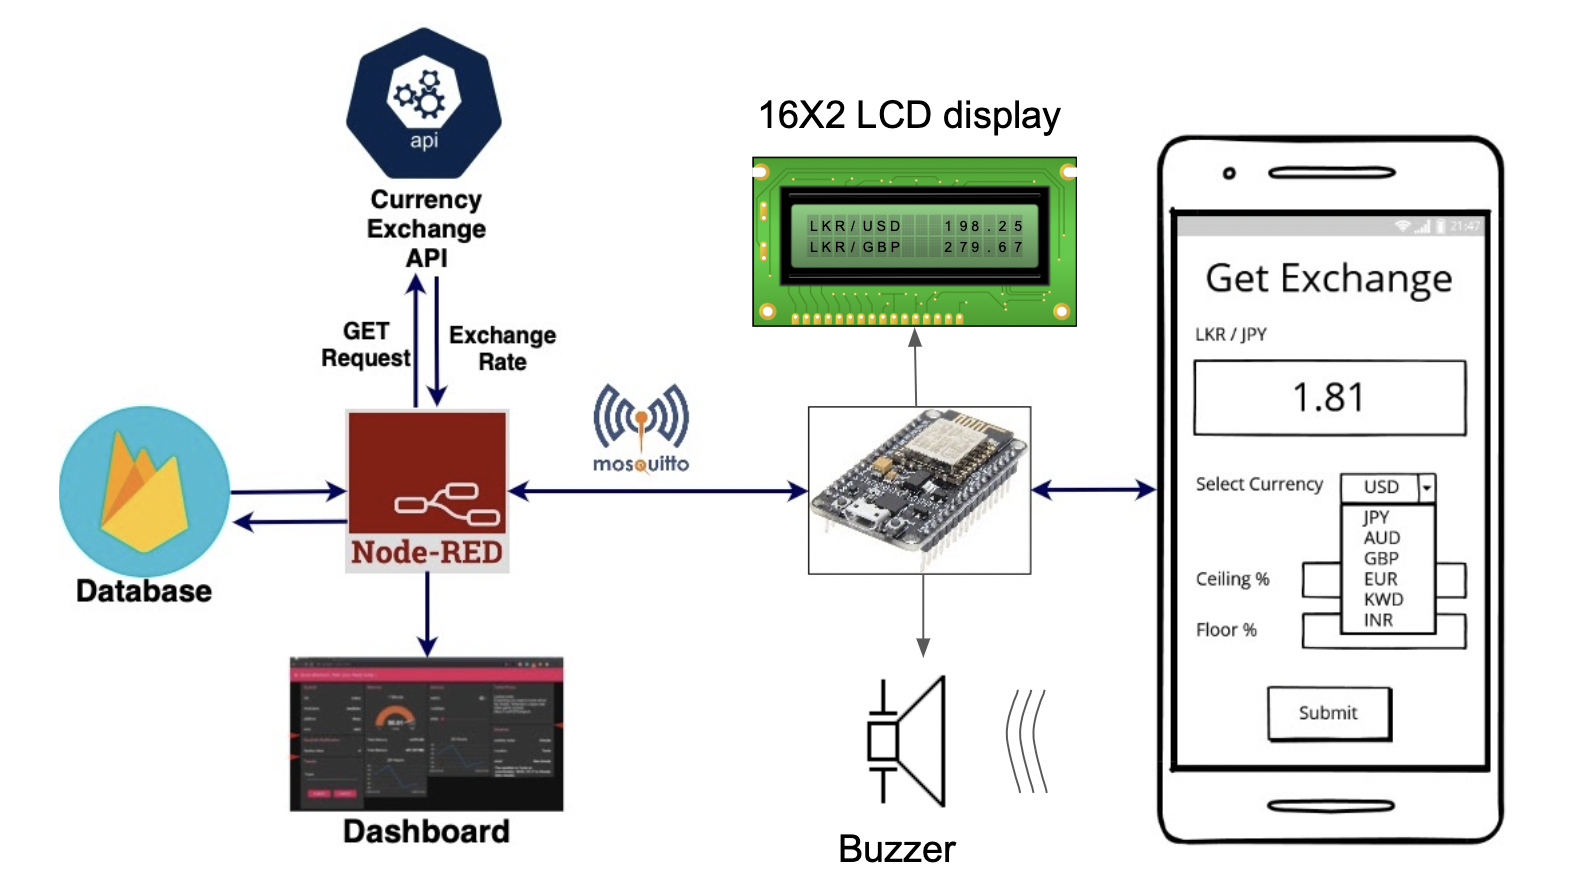
\includegraphics[width=1\textwidth]{images/arch.png}
    \caption{Architecture of Currency Converter Service}
    \label{fig:orgchart}
\end{figure}

\newpage
\bibliographystyle{IEEEbib}
\bibliography{references}


\newpage
\section{Annexes}

\subsection{ESP8266 code}
                
\begin{lstlisting}[language=C++]
{
#if defined(ESP8266)
#include <ESP8266WiFi.h>          
#else
#include <WiFi.h>          
#endif

#if defined(ESP8266)
#include <ESP8266WebServer.h>
#else
#include <WebServer.h>
#endif

#include <WiFiManager.h> 
#include <DNSServer.h>
#include <PubSubClient.h>

#include <WiFiUdp.h>
#include <NTPClient.h>               
#include <TimeLib.h>                 
#include <LiquidCrystal.h>  
LiquidCrystal lcd(D6, D5, D1, D2, D3, D4); 

ESP8266WebServer server(80);

WiFiClient wifiClient;
PubSubClient client(wifiClient); 
const char* mqttServer = "test.mosquitto.org";

// Setup NTP for time and date
WiFiUDP ntpUDP;
NTPClient timeClient(ntpUDP, "asia.pool.ntp.org", 19800, 60000);
char Time[ ] = "TIME:00:00:00";
char Date[ ] = "DATE:00/00/2000";
byte last_second, second_, minute_, hour_, day_, month_;
int year_;
int counter = 0;
unsigned long unix_epoch;
char ascii;

// Node MCU expects from Node-red per 15 seconds
//1) All six currencies values and up/down status ( in the order USD, KWD, AUD, EUR, JPY, GBP)
//2) Selected currency of the user
//3) floor or ceiling exceeded (true/false)


// Node Red expects from Node MCU
//1) Clients selected Currency type
//2) Ceil and Floor of the currency type as percentages (eg-:5,4)
String payloadstr;
unsigned long timestamp;

float USD = 198.25; // up - true, down - false
float GBP = 198.25; // up - true, down - false
float JPY = 198.25; // up - true, down - false
float AUD = 198.25; // up - true, down - false
float KWD = 198.25; // up - true, down - false
float EUR = 198.25; // up - true, down - false

bool usd_up = false;
bool gbp_up = false;
bool jpy_up = false;
bool aud_up = false;
bool kwd_up = false;
bool eur_up = false;
char * binary;

String current_user;
String current_currency;
bool ceil_crossed = false;
bool floor_crossed = false;

//Variables required for buzzer sound
int speakerPin = 13;
int len = 15; // the number of notes
char notes[] = " C C C C C C C C C ";// a space represents a rest
int beats[] = { 1,1, 1, 1, 1, 1, 1, 1, 1, 1, 1, 1, 1, 1, 1, 1, 1, 1, 1 };
int tempo = 300;


void setup_wifi() {
  // Connecting to a WiFi network
  delay(5000);
  WiFiManager wifiManager; 
  wifiManager.autoConnect("IoT6B_G05","12345678");
}

void setupMQTT() {
  client.setServer(mqttServer,1883);
  client.setCallback(callback);
  }

void reconnect() {
  // Loop until we're reconnected
  while (!client.connected()) {
    Serial.print("Attempting MQTT connection...");
    // Create a random client ID
    String clientId = "ESP32Client-";
    clientId += String(random(0xffff), HEX);
    // Attempt to connect
    if (client.connect(clientId.c_str())) {
      Serial.println("connected");
      // Once connected, publish an announcement...
      client.publish("IOT_6B/G05/start", "Hello World");
      // ... and resubscribe
      client.subscribe("IOT_6B/G05/BuzzerNotification");
      client.subscribe("IOT_6B/G05/CommonData");
    } else {
      Serial.print("failed, rc=");
      Serial.print(client.state());
      Serial.println(" try again in 500 milli seconds");
      // Wait 5 seconds before retrying
      delay(500);
    }
  }
}

void setup() {
  // put your setup code here, to run once:
  
  lcd.begin(16, 2);                 // Initialize 16x2 LCD Display
  lcd.clear();
  lcd.setCursor(0, 0);
  lcd.print(Time);
  lcd.setCursor(0, 1);
  lcd.print(Date);
  timeClient.begin();

  pinMode(speakerPin, OUTPUT);  // Output pin for buzzer
  
  pinMode(BUILTIN_LED, OUTPUT);     // Initialize the BUILTIN_LED pin as an output
  WiFi.mode(WIFI_AP_STA);
  Serial.begin(115200);
  setup_wifi();
  setupMQTT();

  //client.subscribe("IOT_6B/G05/Response");
  //client.subscribe("IOT_6B/G05/ceil");
  
  server.on("/",handlerequest);
  server.onNotFound(handle_NotFound);

  server.begin();
  Serial.println("HTTP server started");

}

void loop() {
  server.handleClient();
  if (!client.connected()) {
    reconnect();
  }
  client.loop();

    timeClient.update();
  unix_epoch = timeClient.getEpochTime();    // Get Unix epoch time from the NTP server
  //Serial.println(unix_epoch);
  second_ = second(unix_epoch);
  if (last_second != second_) {
 

    minute_ = minute(unix_epoch);
    hour_   = hour(unix_epoch);
    day_    = day(unix_epoch);
    month_  = month(unix_epoch);
    year_   = year(unix_epoch);

    Time[12] = second_ % 10 + 48;
    Time[11] = second_ / 10 + 48;
    Time[9]  = minute_ % 10 + 48;
    Time[8]  = minute_ / 10 + 48;
    Time[6]  = hour_   % 10 + 48;
    Time[5]  = hour_   / 10 + 48;

    Date[5]  = day_   / 10 + 48;
    Date[6]  = day_   % 10 + 48;
    Date[8]  = month_  / 10 + 48;
    Date[9]  = month_  % 10 + 48;
    Date[13] = (year_   / 10) % 10 + 48;
    Date[14] = year_   % 10 % 10 + 48;

    //Serial.println(Time);
    //Serial.println(Date);

    lcd.setCursor(0, 0);
    lcd.print(Time);
    lcd.setCursor(0, 1);
    lcd.print(Date);
    last_second = second_;

  }
  delay(500);

  if (counter == 8){
    counter = 0;
    lcd.setCursor(0, 0);
    lcd.print("LKR/USD "+ String(USD));
    lcd.setCursor(0, 1);
    lcd.print("LKR/GBP "+ String(GBP));

    if (usd_up){
      ascii = 0x5e;
      lcd.setCursor(15 , 0);
      lcd.print(ascii);
    } else {
      ascii = 0x76;
      lcd.setCursor(15 , 0);
      lcd.print(ascii);
    }

    if (gbp_up){
      ascii = 0x5e;
      lcd.setCursor(15 , 1);
      lcd.print(ascii);
    } else {
      ascii = 0x76;
      lcd.setCursor(15 , 1);
      lcd.print(ascii);
    }
    delay(2000);

    server.handleClient();
    client.loop();

    
    lcd.clear();
    lcd.setCursor(0, 0);
    lcd.print("LKR/JPY   "+ String(JPY));
    lcd.setCursor(0, 1);
    lcd.print("LKR/AUD "+ String(AUD));

    if (jpy_up){
      ascii = 0x5e;
      lcd.setCursor(15 , 0);
      lcd.print(ascii);
    } else {
      ascii = 0x76;
      lcd.setCursor(15 , 0);
      lcd.print(ascii);
    }

    if (aud_up){
      ascii = 0x5e;
      lcd.setCursor(15 , 1);
      lcd.print(ascii);
    } else {
      ascii = 0x76;
      lcd.setCursor(15 , 1);
      lcd.print(ascii);
    }
    delay(2000);

    server.handleClient();
    client.loop();
    lcd.clear();
    lcd.setCursor(0, 0);
    lcd.print("LKR/KWD "+ String(KWD));
    lcd.setCursor(0, 1);
    lcd.print("LKR/EUR "+ String(EUR));

    if (kwd_up){
      ascii = 0x5e;
      lcd.setCursor(15 , 0);
      lcd.print(ascii);
    } else {
      ascii = 0x76;
      lcd.setCursor(15 , 0);
      lcd.print(ascii);
    }

    if (eur_up){
      ascii = 0x5e;
      lcd.setCursor(15 , 1);
      lcd.print(ascii);
    } else {
      ascii = 0x76;
      lcd.setCursor(15 , 1);
      lcd.print(ascii);
    }

    delay(2000);
    server.handleClient();
    client.loop();
    lcd.clear();
  } else {
    counter += 1;
  }

}

void handlerequest(){
//  if (server.hasArg("plain")== false){ //Check if body received
//      server.send(200, "text/plain", "Body not received");
//      return;
//      }
      String UserNeeds;
      current_currency = server.arg("currency");
      String Ceil = server.arg("ceil");
      String Floor = server.arg("floor");
      unsigned long timenow = unix_epoch - 19800;

      UserNeeds  = timenow + "$" + current_currency +"$"+ Ceil +"$"+ Floor;



      int currency_len = current_currency.length() ;
      int ceil_len = Ceil.length();
      int floor_len = Floor.length(); 
      
      int UserNeeds_len = currency_len + ceil_len + floor_len +3;

      char UserNeeds_array[UserNeeds_len];
      UserNeeds.toCharArray(UserNeeds_array, UserNeeds_len);
      client.publish("IOT_6B/G05/UserNeeds", UserNeeds_array );


      server.send(200, "text/html", SendHTML(current_currency));
}

void handle_NotFound(){
  server.send(404, "text/plain", "Not found");
}

String SendHTML(String Currency){
  String ptr = "<!DOCTYPE html> <html lang=\"en\">\n";
  ptr+= "<head>\n";
  ptr+= "<link rel=\"stylesheet\" href=\"https://cdnjs.cloudflare.com/ajax/libs/font-awesome/4.7.0/css/font-awesome.min.css\">\n";   
  ptr+= "<meta charset=\"UTF-8\">\n";
  ptr+= "<meta http-equiv=\"X-UA-Compatible\" content=\"IE=edge\">\n";
  ptr+= "<meta name=\"viewport\" content=\"width=device-width, initial-scale=1.0\">\n";
  ptr+= "<title>GROUP 5</title>\n";
  ptr+= "</head>\n";
  ptr+= "<body style=\"text-align:center;display:grid;place-content: center;background-color: rgb(23, 196, 196);\"\n";
  ptr+= "<h1 style=\"font-size: 200px;\" >Get Exchange</h1>\n";
  
  if (Currency == "USD"){
    ptr+="<h2>LKR/USD</h2>\n";
  }
  else if (Currency == "JPY"){
    ptr+="<h2>LKR/JPY</h2>\n";
  }
  else if (Currency == "GBP"){
    ptr+="<h2>LKR/GBP</h2>\n";
  }
  else if (Currency == "EUR"){
    ptr+="<h2>LKR/EUR</h2>\n";
  }
  else if (Currency == "KWD"){
    ptr+="<h2>LKR/KWD</h2>\n";
  }
  else if (Currency == "INR"){
    ptr+="<h2>LKR/INR</h2>\n";
  }
  else{
    ptr+="<h2>LKR/NON</h2>\n";
  }
  
  ptr+= "<h1 style=\" color :rgb(62, 128, 0)\">1.81 <i class=\"fa fa-arrow-up\"></i></h1>\n";
  ptr+= "<h1 style=\" color :red\">1.81 <i class=\"fa fa-arrow-down\"></i></h1>\n";
  ptr+= "<form name=\"dropdown\" method=\"get\" style=\" font-size: xx-large;\" >\n";
  ptr+= "<label for=\"currency_label\">Select Currency :</label><br>\n";
  ptr+= "<select name=\"currency\" id=\"currency\">\n";
  ptr+= "<option value=\"USD\">USD</option>\n";
  ptr+= "<option value=\"JPY\">JPY</option>\n";
  ptr+= "<option value=\"GBP\">GBP</option>\n";
  ptr+= "<option value=\"EUR\">EUR</option>\n";
  ptr+= "<option value=\"KWD\">KWD</option>\n";
  ptr+= "<option value=\"INR\">INR</option>\n";
  ptr+= "</select>\n";
  ptr+= "<br><br>\n";
  ptr+= "<label for=\"ceil\">Ceil% :</label><br>\n";
  ptr+= "<input type=\"number\" id=\"ceil\" name=\"ceil\" value=5><br><br>\n";
  ptr+= "<label for=\"floor\">Floor% :</label><br>\n";
  ptr+= "<input type=\"number\" id=\"floor\" name=\"floor\" value=5><br><br>\n";
  ptr+= "<input type=\"submit\" value=\"Submit\">\n";
  ptr+= "</form>\n";
  ptr+= "</body>\n";
  ptr+= "</html>\n";
  return ptr;
}

void callback(char* topic, byte* payload, unsigned int length) {

  if (String(topic) == "IOT_6B/G05/BuzzerNotification") {
   process_notification(payload, length, 50, 5);
  }
  
  if (String(topic) == "IOT_6B/G05/CommonData") {
   process_data(payload, length, 70, 8);
  }

  if (ceil_crossed  || floor_crossed) {
    buzzerinit();  
    ceil_crossed = false;
    floor_crossed = false;
  }
}

void process_notification(byte* payload, unsigned int length, int charlen, int numitem) {

    int digit;
    payloadstr = "";
    Serial.println();
    for (int i = 0; i < length; i++) {
      payloadstr += (char)payload[i];
    }

     char payloadstr_array[charlen];
     payloadstr.toCharArray(payloadstr_array, charlen);

   char * token = strtok(payloadstr_array, "$");
   
   for (int i = 1; i < numitem+1; i++) {
      switch (i) {
       case 1:
          timestamp = atol(token);
          Serial.print(timestamp);
          Serial.println();
          break;
       case 2:
          if (timestamp > unix_epoch - 19820) {
           current_user = String(token);
           Serial.print(current_user);
           Serial.println();
          }
           break;
       case 3:
          if (timestamp > unix_epoch - 19820) {
           current_currency = String(token);
           Serial.print(current_currency);
           Serial.println();
          }
           break;
       case 4:
          if (timestamp > unix_epoch - 19820) {
           digit = String(token).toInt();
           if (digit == 1) {
           ceil_crossed = true;
            } else {
            ceil_crossed  = false;
            }
           Serial.print(ceil_crossed);
           Serial.println();
          }
          break;
       case 5:
          if (timestamp > unix_epoch - 19820) {
           digit = String(token).toInt();
           if (digit == 1) {
           floor_crossed = true;
            } else {
           floor_crossed  = false;
            }
           Serial.print(ceil_crossed);
           Serial.println();
          }
          break;    
       }
       token = strtok(NULL, "$");
   }
}

void process_data(byte* payload, unsigned int length, int charlen, int numitem) {

    payloadstr = "";
    Serial.println();
    for (int i = 0; i < length; i++) {
      payloadstr += (char)payload[i];
    }

     char payloadstr_array[charlen];
     payloadstr.toCharArray(payloadstr_array, charlen);

   char * token = strtok(payloadstr_array, "$");

   for (int i = 1; i < numitem+1; i++) {
      switch (i) {
       case 1:
          timestamp = atol(token);
          Serial.print(timestamp);
          Serial.println();
          break;
       case 2:

           USD = String(token).toFloat();
           Serial.print(USD);
           Serial.println();
           break;
       case 3:

           GBP = String(token).toFloat();
           Serial.print(GBP);
           Serial.println();
           break;
       case 4:

           JPY = String(token).toFloat();
           Serial.print(JPY);
           Serial.println();
          break;
       case 5:

           AUD = String(token).toFloat();
           Serial.print(AUD);
           Serial.println();
          break;
       case 6:
          //do something when var equals 1
           KWD = String(token).toFloat();
           Serial.print(KWD);
           Serial.println();
          break;
       case 7:

           EUR = String(token).toFloat();
           Serial.print(EUR);
           Serial.println();
          break;
       case 8:
           set_updown(token);
           break;        
       }
       token = strtok(NULL, "$");
   }

}

void set_updown(char * binary) {
  int digit;
  for (int i = 1; i < 7; i++) {
    switch (i) {
       case 1:
       digit = String((char)binary[i-1]).toInt();
       if (digit == 1) {
        usd_up = true;
       } else {
        usd_up = false;
       }
       Serial.print(usd_up);
       Serial.println();
       break;

       case 2:
       digit = String((char)binary[i-1]).toInt();
       if (digit == 1) {
        gbp_up = true;
       } else {
        gbp_up = false;
       }
       Serial.print(gbp_up);
       Serial.println();
       break;

       case 3:
       digit = String((char)binary[i-1]).toInt();
       if (digit == 1) {
        jpy_up = true;
       } else {
        jpy_up = false;
       }
       Serial.print(jpy_up);
       Serial.println();
       break;

       case 4:
       digit = String((char)binary[i-1]).toInt();
       if (digit == 1) {
        aud_up = true;
       } else {
        aud_up = false;
       }
       Serial.print(aud_up);
       Serial.println();
       break;

       case 5:
       digit = String((char)binary[i-1]).toInt();
       if (digit == 1) {
        kwd_up = true;
       } else {
        kwd_up = false;
       }
       Serial.print(kwd_up);
       Serial.println();
       break;

       case 6:
       digit = String((char)binary[i-1]).toInt();
       if (digit == 1) {
        eur_up = true;
       } else {
        eur_up = false;
       }
       Serial.print(eur_up);
       Serial.println();
       break;
    }
  }
}

void playTone(int tone, int duration) {
  for (long i = 0; i < duration * 1000L; i += tone * 2) {
    digitalWrite(speakerPin, HIGH);
    delayMicroseconds(tone);
    digitalWrite(speakerPin, LOW);
    delayMicroseconds(tone);
  }
}

void playNote(char note, int duration) {
  char names[] = { 'c', 'd', 'e', 'f', 'g', 'a', 'b', 'C' };
  int tones[] = { 1915, 1700, 1519, 1432, 1275, 1136, 1014, 956 };

  // play the tone corresponding to the note name
  for (int i = 0; i < 8; i++) {
    if (names[i] == note) {
      playTone(tones[i], duration);
    }
  }
}

void buzzerinit() {
  for (int i = 0; i < len; i++) {
    if (notes[i] == ' ') {
      delay(beats[i] * tempo); // rest
    } else {
      playNote(notes[i], beats[i] * tempo);
    }

    // pause between notes
    delay(tempo / 2); 
  }
}
}
\end{lstlisting}

\subsection{JavaScript codes used in Node-Red}




\end{document}
